% Author: Izaak Neutelings (August 2021)
\documentclass[border=3pt,tikz]{standalone}
\usepackage{tikz}
\usepackage{ifthen}
\tikzset{>=latex} % for LaTeX arrow head

\def\ltick{0.09} % tick length
\def\xtick#1#2{\draw[thick] (#1)++(90:\ltick) --++ (-90:2*\ltick) node[below=-2,scale=0.9] {#2};}
\def\ytick#1#2{\draw[thick] (#1)++(0:\ltick) --++ (180:2*\ltick) node[left=-2,scale=0.9] {#2};}

\begin{document}


% 2D SCAN
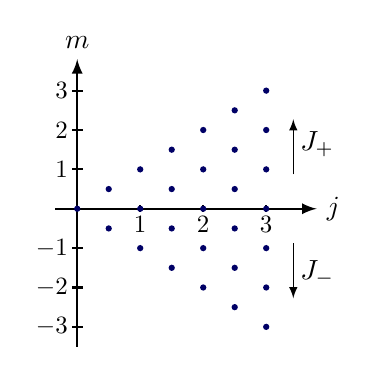
\begin{tikzpicture}[x=0.8cm,y=0.5cm]
  \def\N{3} % number of horizontal (m) points
  \def\xmax{3.5} % axis length
  \def\ymax{3.5} % axis length
  \def\xs{1} % x scale
  \def\ys{1} % y scale
  \def\r{0.04} % radius dot
  
  % AXES
  \draw[->,thick] (-0.1*\xmax,0) -- (\xmax+0.3,0) node[right] {$j$};  
  \draw[->,thick] (0,-\ymax) -- (0,\ymax+0.3) node[above] {$m$};
  
  % ARROWS
  \draw[->] (0.98*\xmax,0.25*\ymax) --++ (0,0.4*\ymax)
    node[pos=0.55,right=-1] {$J_+$};
  \draw[->] (.98*\xmax,-0.25*\ymax) --++ (0,-0.4*\ymax)
    node[pos=0.55,right=-1] {$J_-$};
  
  % DOTS
  \fill[black!60!blue] (0,0) circle (\r cm);
  \foreach \j [evaluate={\x=\xs*\j; \y=\ys*\j;}] in {1,...,\N}{
    \xtick{\x,0}{\j};
    \ytick{0,\y}{\j};
    \ytick{0,-\y}{$-\j$};
    \foreach \m [evaluate={\ym=\ys*\m;}] in {-\j,...,\j}{
      \fill[black!60!blue] (\x,\ym) circle (\r cm);
      \ifthenelse{\m < \j}{
        \fill[black!60!blue] ({\x-\xs/2},{\ym+\ys/2}) circle (\r cm);
      }{}
    }
  }
  
\end{tikzpicture}


\end{document}